%%%%%%%%%%%%%%%%%%%%%%%%%%%%%%%%%%%%%%%%%%%%%%%%%%%%%%%%%%%%%%%%%%%%%%%
%% Zusammenfassung und Ausblick
\section{Implementierung}
\label{sec:impl}

In diesem Kapitel werden einige Aspekte der Entwicklung aufgegriffen und im Detail ausgeführt. Der Name Implementierung bezieht sich nicht auf die Programmierung, sondern die Umsetzung von Schnittstellen und den Algorithmen hinter speziellen Problemen. So wird zum Beispiel in dem Unterkapitel \ref{sec:impl-rs} auf die Bewegung auf einer linearen Trajektorie eingegangen. Außerdem werden Probleme beschrieben und gelöst, die während der Umsetzung der Konzepte auftraten. Des Weiteren werden die genutzten Bibliotheken erwähnt und die Anbindung von ROS an die Konzepte. Den zentralen Aspekt in diesem Kapitel stellt jedoch Unterkapitel \ref{sec:impl-hop} dar. In diesem wird die Bestimmung für die Übergabeposition vorgestellt.

\subsection{Robotersteuerung - RATSYoubot \& RATSDummy \& RATSRose}
\label{sec:impl-rs}
In diesem Kapitel wird die Ansteuerung für die Roboter und deren Arme vorgestellt. Diese beruht vor allem auf der Kuka API für den Youbot. Außerdem wird die Bewegung auf einer linearen Trajektorie, sowie die einzelnen Aktionen die ein Roboter ausführen kann kurz aufgelistet und beschrieben.

\subsubsection{Ansteuerung der Aktoren}
\label{sec:impl-res-ak}
Die Aktoren innerhalb der Roboter werden mit Hilfe von ROS Topics angesteuert. Diese werden von dem Controllernode \textit{youbot\_driver} ausgelesen und in die Steuersignale für die Motoren umgewandelt. Für die Ansteuerung des Arms existieren zwei Topics. Der \textit{velocity\_command}-Topic erwartet für jedes Gelenk eine Geschwindigkeitsangabe. Für diese Arbeit wird jedoch mit Positionsangaben gearbeitet. Der dazu gehörige Topic \textit{arm\_controller/position\_command} benötigt ein Array mit Gelenkkonfigurationen. Dafür wird die ROS-Bibliothek \textit{BRICS} genutzt. Diese beinhaltet Nachrichten für inverse Kinematiken, wie zum  Beispiel: Posen, Vektoren und Rotationen im Kartesischen Raum oder Aktoren Nachrichten, wie Gelenkeinstellung, Gelenkgeschwindigkeiten und Gelenkbeschleunigungen. Neben der Armansteuerung gibt es für die Gripper eine eigene Topic \textit{gripper\_controller/position\_command}. Dieser transportiert ebenfalls Gelenkeinstellungen. Dabei kann die Position der einzelnen Finger des Grippers angegeben werden. Die Werte entsprechen dabei der Distanz der Finger zu ihrer Basisposition. Ein Nachteil der Ansteuerung über die Topics ist das fehlende Feedback. Der Absender erfährt nicht, ob das Signal angekommen ist und wann die Bewegung beendet ist. Sollen Bewegungen seriell ausgeführt werden muss der ausführende Thread blockiert werden, bis die Gelenke die Zielkonfiguration erreicht haben.  Ein paralleler Thread liest die aktuelle Gelenkkonfiguration aus und berechnet eine Differenz für jedes einzelne Gelenk und die Quadratsumme über alle Gelenke. Solange die Differenz für mindestens ein Gelenk oder die Summe der Quadrate ihre Schwellwerte überschreiten blockiert ein Mutex den ausführenden Thread. Ein weiteres Problem während der Implementierung stellte die Ungenauigkeit der Ansteuerung dar. Dabei kam es großen Abweichungen an einem Gelenk, wenn es eine große Winkeländerung hatte. Dieses Überschlagen lässt sich auf die Massenträgheit des Armes und dem abrupten Abbremsen der Motoren zurückführen. Dies konnte jedoch auch durch den parallelen Thread abgefangen werden. Dieser überprüft nun auch neben der Distanz zu der Zieleinstellung, die Distanz zur letzten gemessenen Gelenkeinstellung. Ist diese nahe null, also der Arm nicht mehr in Bewegung, und die Distanz zum Ziel zu groß wurde nochmal die selbe Gelenkeinstellung an den Motorencontroller geschickt.

Die Ansteuerung der mobilen Plattform wird mit einer einzelnen Topic \textit{cmd\_vel} umgesetzt. Dabei wird eine einzelne Nachricht übermittelt. Diese beinhaltet eine Twist Nachricht aus dem \textit{geometry\_msg} Paket. In dieser Nachricht kann eine lineare und eine Winkelgeschwindigkeit angegeben werden. Diese können für die einzelnen Achsen zerlegt werden. Für die mobile Plattform werden jedoch nur die X- und Y- Achsen der linearen, sowie die Z-Achse der Rotationsgeschwindigkeit ausgelesen und als absoluten Wert gesetzt. Der Controller rechnet anschließend die benötigten Steuersignale für die einzelnen Räder und Motoren aus.

\subsubsection{Lineare Bahnbewegung}
\label{sec:impl-res-lb}
Die lineare Bahnbewegung wird beim Aufheben, Ablegen und während der Übergabe benötigt. Dies liegt vor allem an der Kollisionsvermeidung des Objektes mit der Umwelt. Da die inverse Kinematik die Gelenkeinstellungen und nicht die Gelenkgeschwindigkeiten berechnet ist es nicht so einfach auf einer gezielten Trajektorie entlang zufahren. Der Übergang zwischen zwei Gelenkeinstellung wird nicht genau definiert. Wie in Abbildung \ref{fig:traj} dargestellt kommt es dabei durch unterschiedliche Gelenkgeschwindigkeiten zu einem Ausschlagen des Greifers. Je größer die Distanz zwischen zwei Posen, desto größer der Ausschlag. Deshalb kann dies verhindert beziehungsweise minimiert werden, indem Zwischenposen auf der Trajektorie ermittelt werden, die nacheinander angefahren werden. Dies erfordert zwar eine häufiges Aufrufen der inversen Kinematik, dafür kann eine Trajektorie mit einem geringen Ausschlag entlang gefahren werden. Tests mit dem YouBot Armen und der inversen Kinematik ergaben eine Distanz von 5 Millimetern zwischen den Zwischenposen als optimal. Bei einer kleineren Distanz reduzierte sich die Amplitude des Ausschlages weniger als vorher und steigert die Kosten durch einen häufigeren Aufruf der inversen Kinematik. Bei der Implementierung nutzt dafür vor allem die Orocos KDL Api, die auch bei der Implementierung der inversen Kinematik genutzt wird. Diese ermöglicht das Rechnen mit geometrischen Primitiven, so wurde der \lstinline|KDL::Frame| für die Abbildung von Koordinatensystemen und Posen genutzt. Dieser ermöglicht unter anderem die Bestimmung der Zwischenposen.

\begin{figure}[h]
	\centering
	\subfigure[]{%
		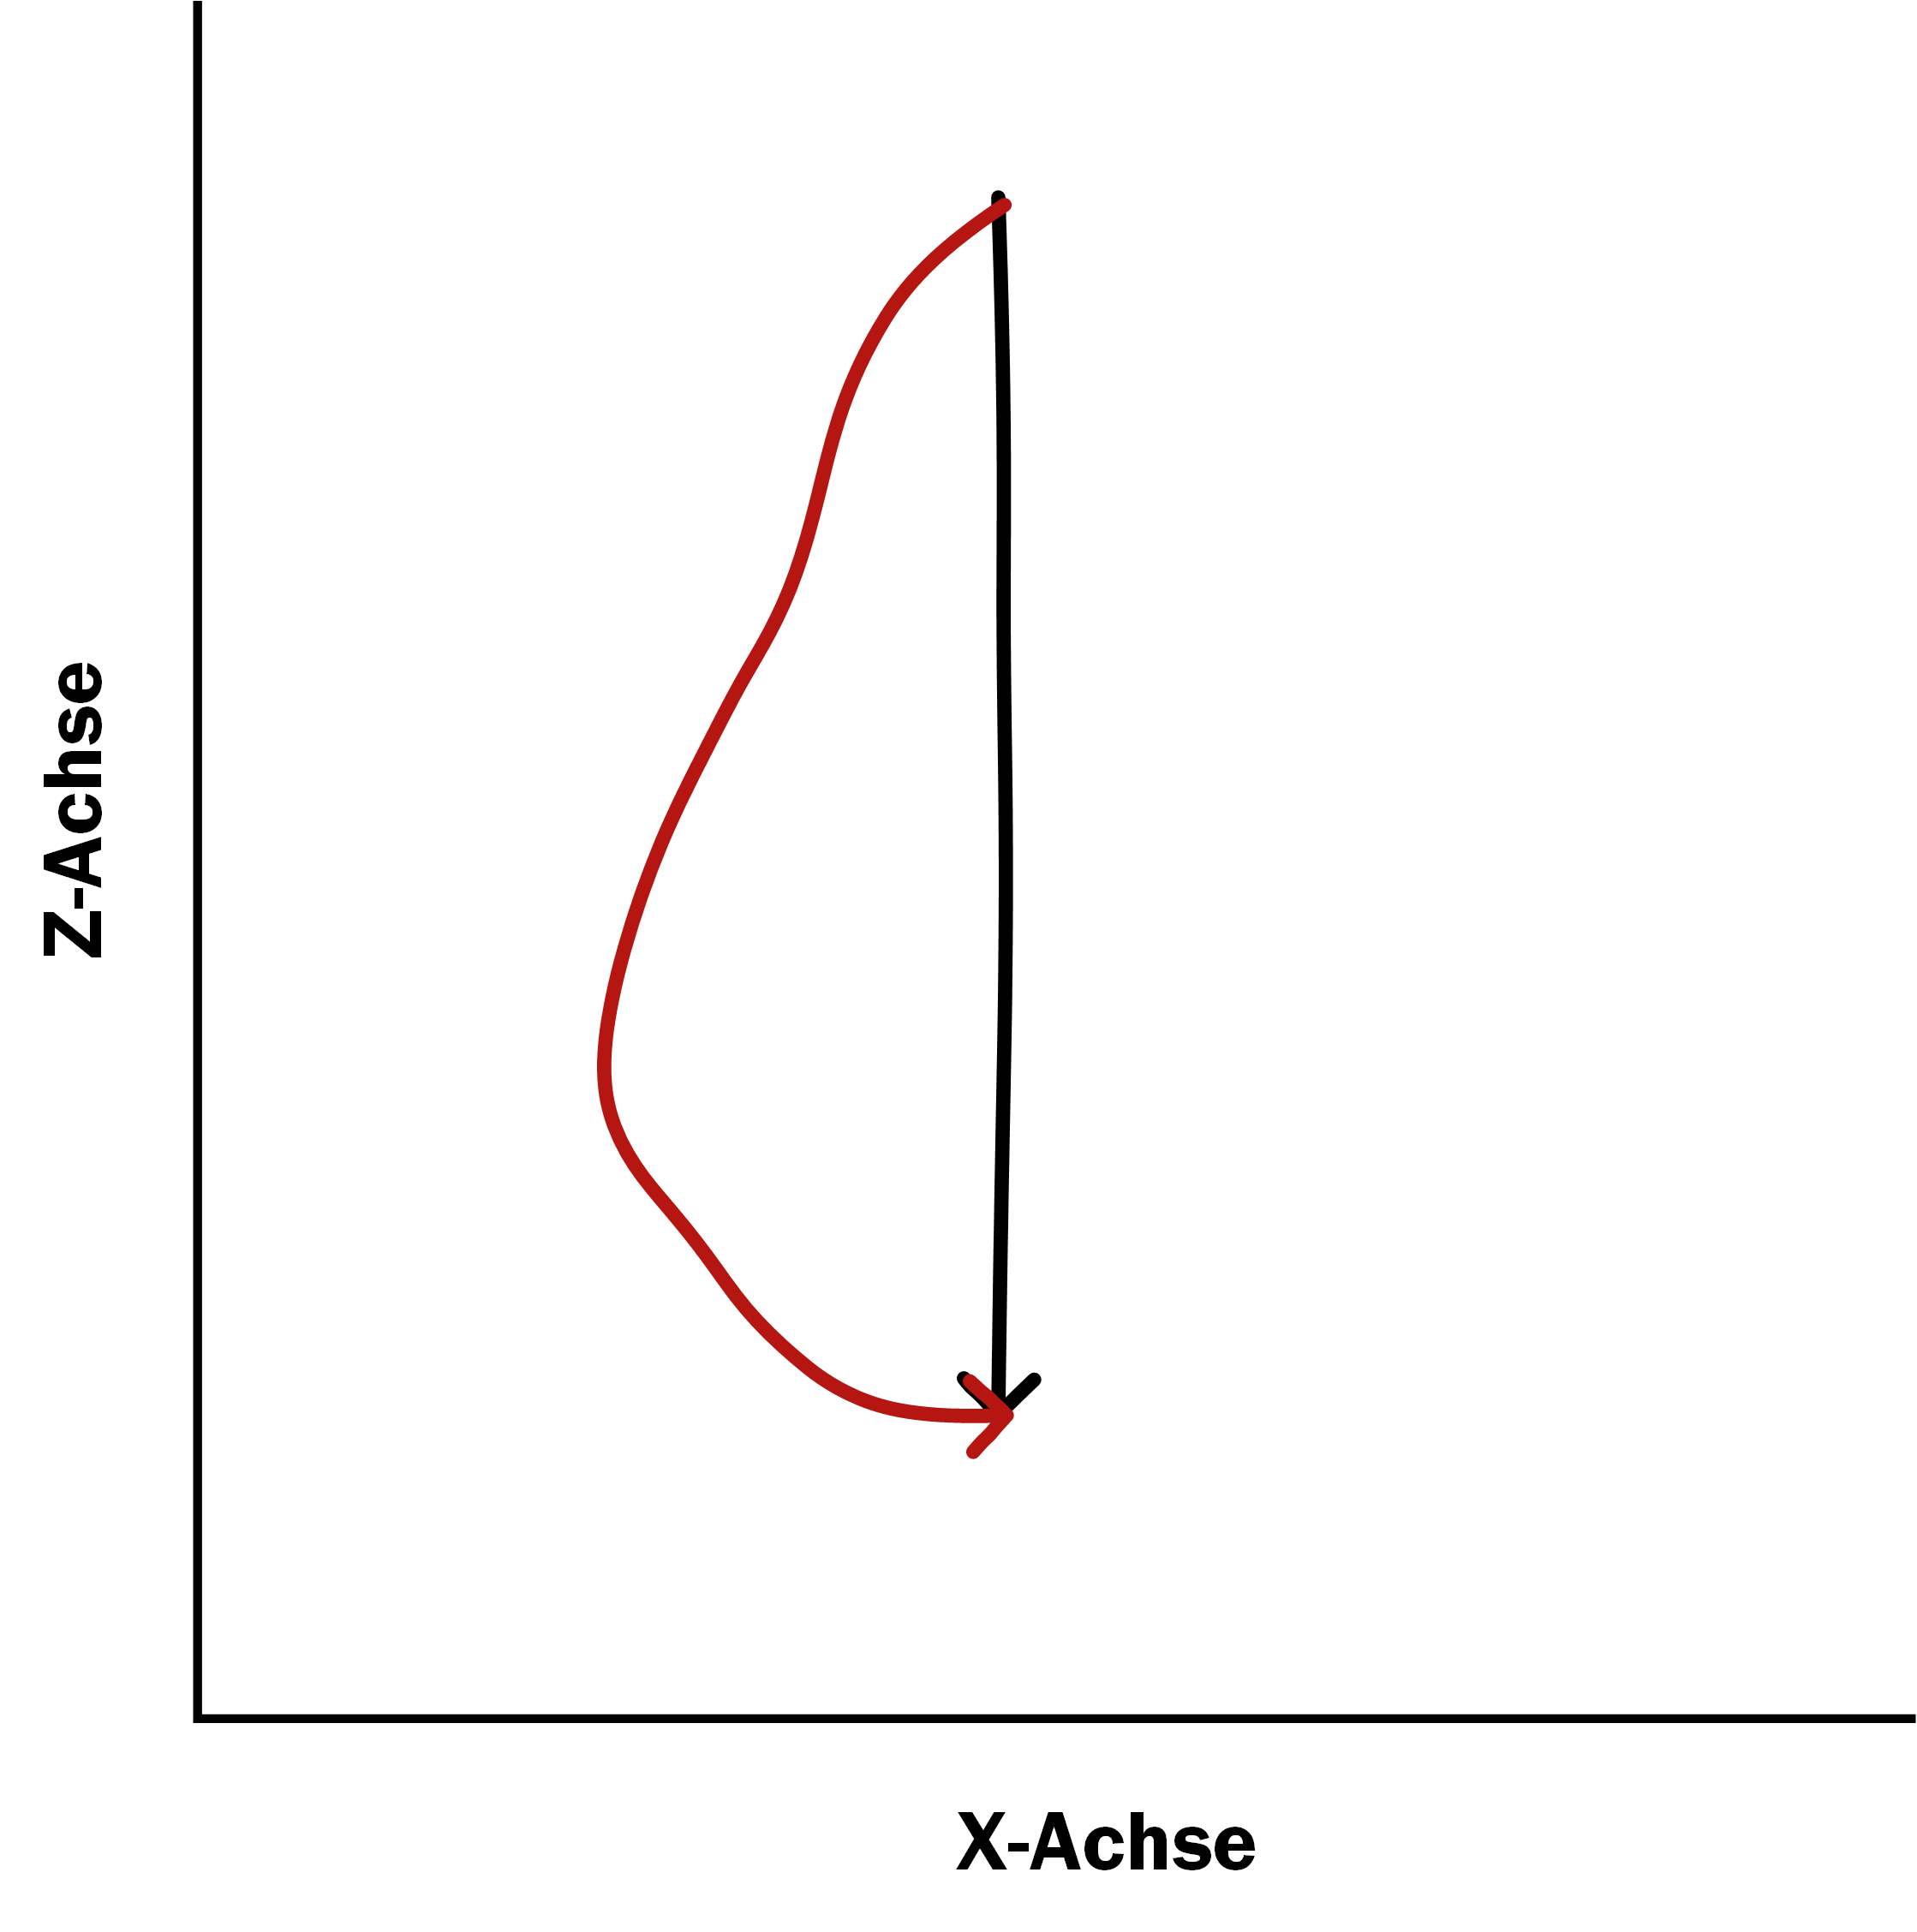
\includegraphics[scale=0.7]{fig/traj1}}
	\hfill
	\subfigure[]{%
		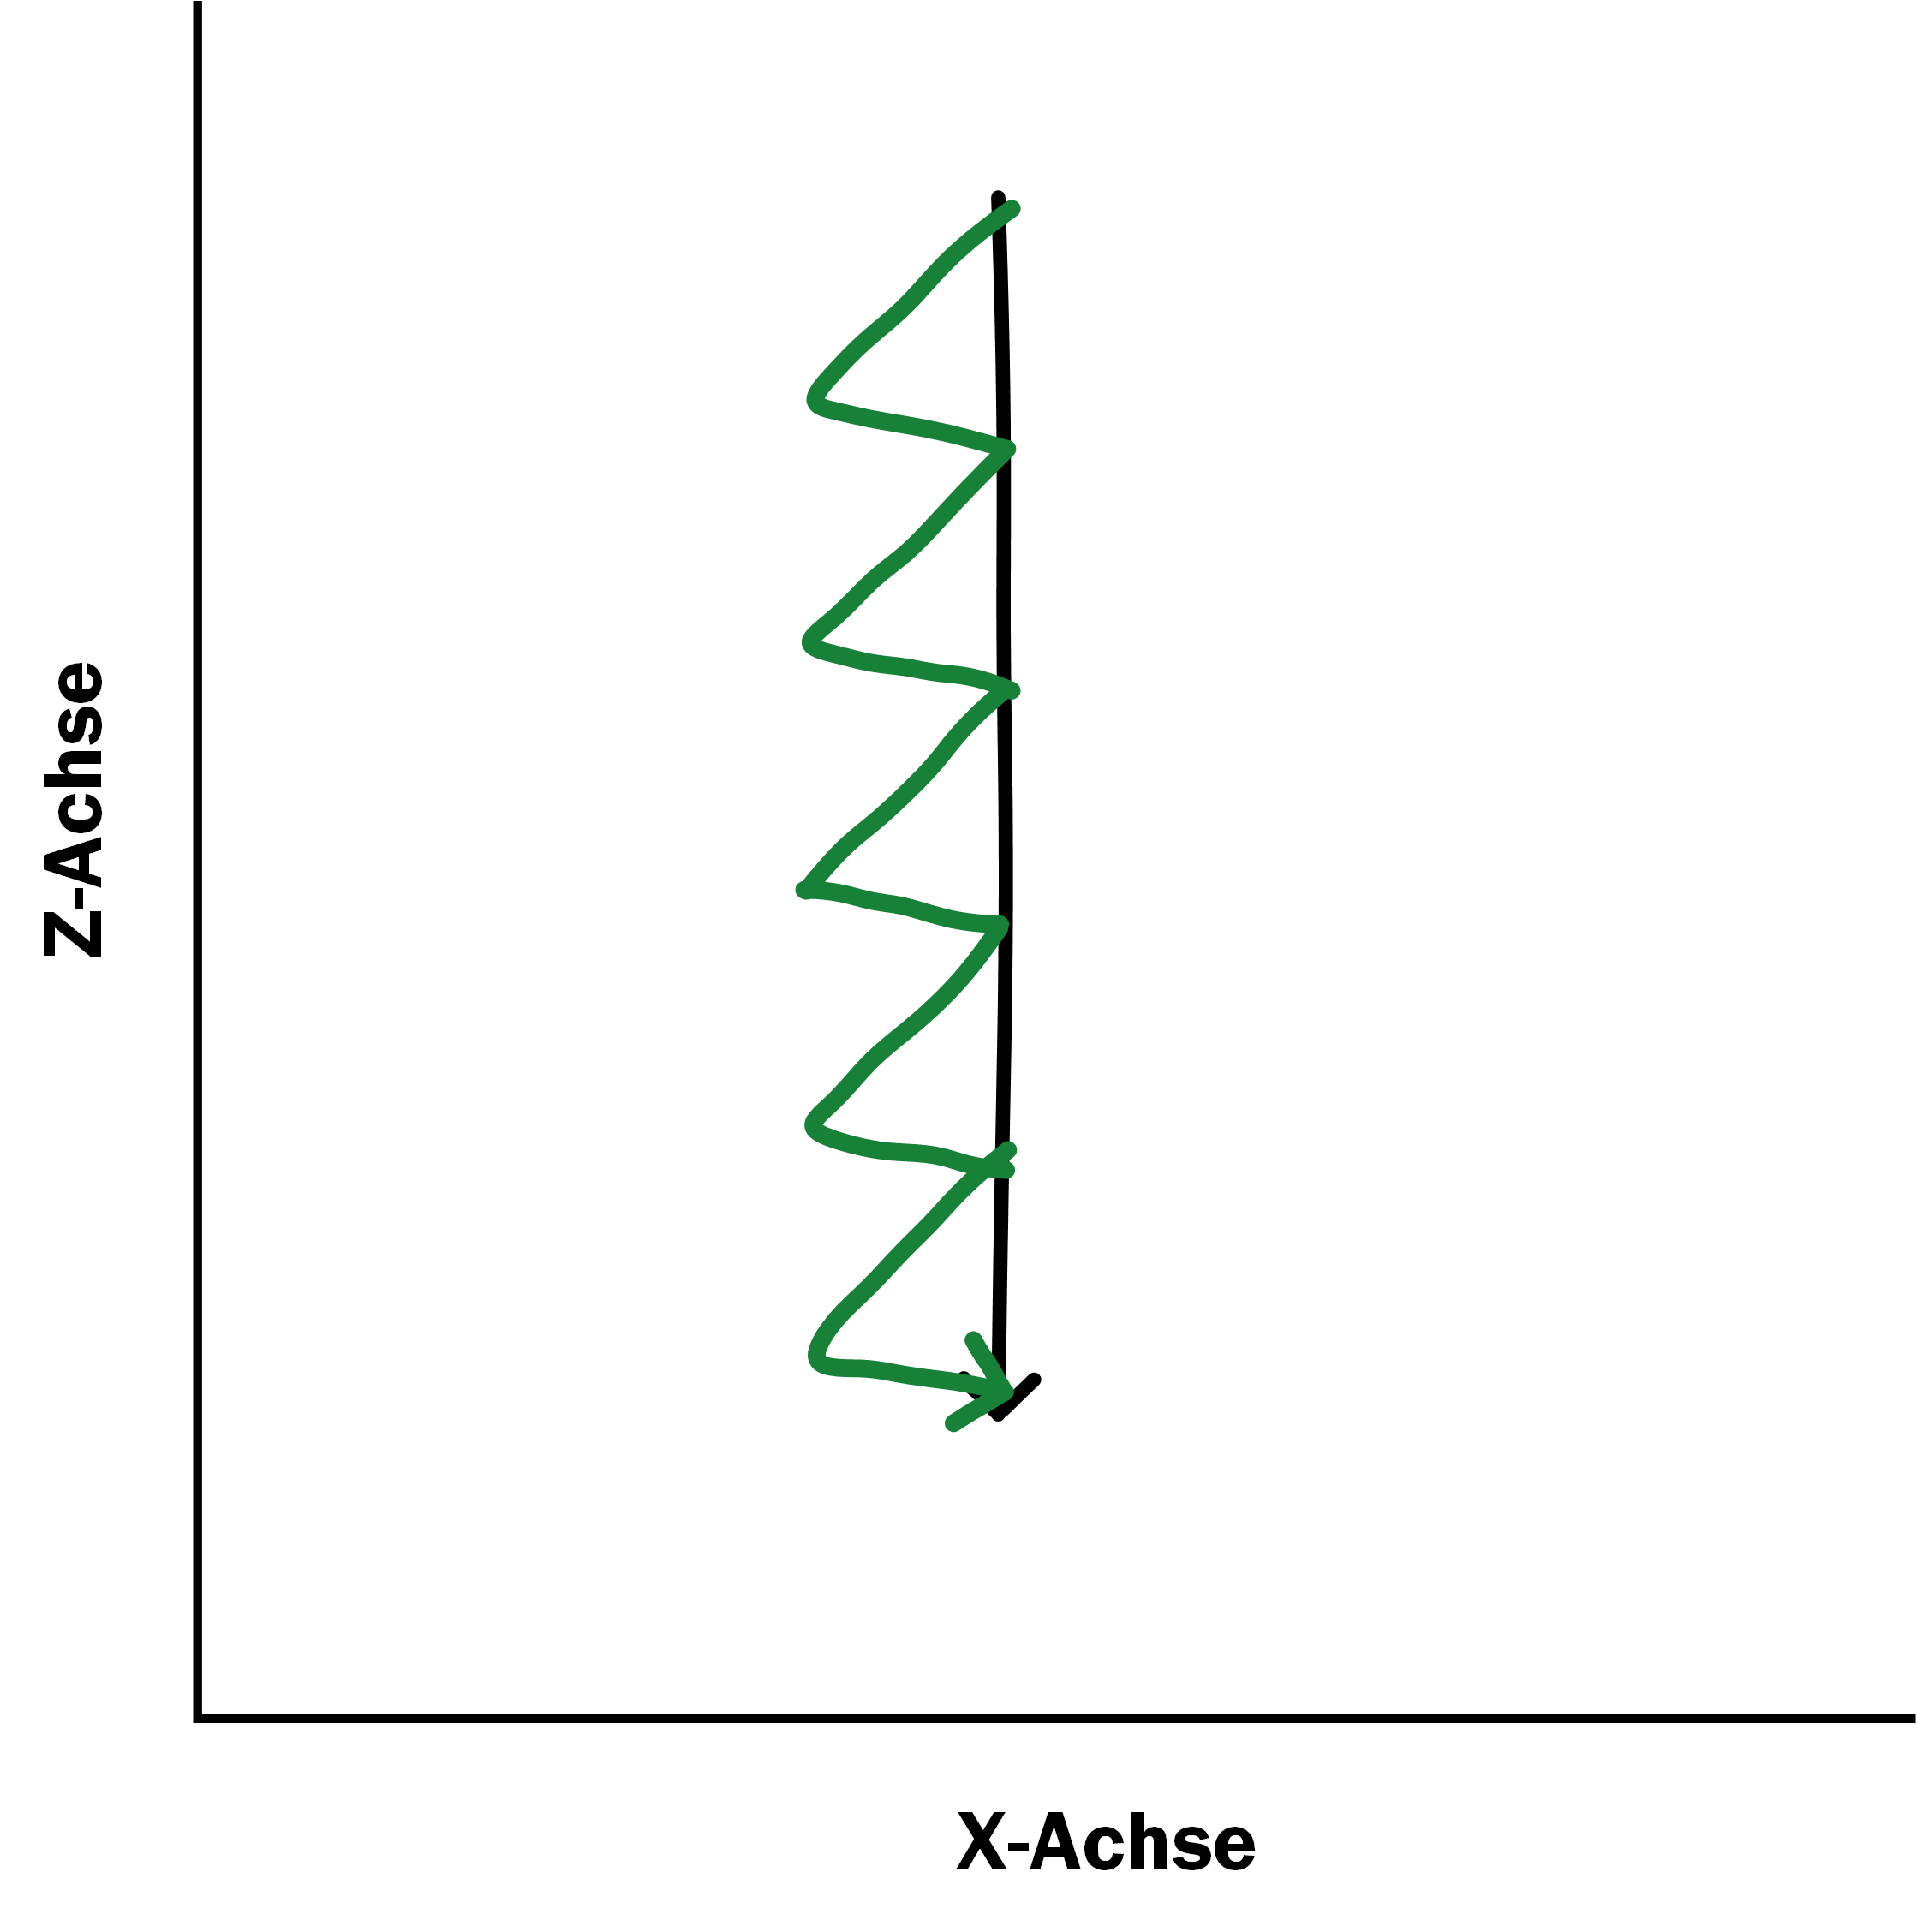
\includegraphics[scale=0.7]{fig/traj2}}
	\caption[Trajektorien des Greifers]{Die dargestellten Graphen stellen die gewünschte Trajektorie (schwarz) und die realen Trajektorien des Greifers dar. Dabei handelt es sich um eine lineare Absenkung auf der Z-Achse. Links: Trajektorie (rot) bei Angabe der Zielpose. Rechts: Trajektorie (grün) bei Angabe von Zwischenposen auf der gewünschten Trajektorie. Bildquelle: \cite{muggler2013torque}}	
	\label{fig:traj}
\end{figure}

\subsubsection{Aktionen der Roboter}

In diesem Unterkapitel wird sehr kurz auf die Aktionen eingegangen, die für die Roboter implementiert wurden. Aus Gründen des Umfangs wird dabei auf Grafiken, wie zum Beispiel UML-Diagramme, verzichtet. Aktionen die nur für einen Roboter implementiert wurden, sind speziell gekennzeichnet.

\paragraph{Greifer öffnen und schließen} Diese Aktion sind eigentlich zwei. Für beide Roboter wurde eine Aktion für das Öffnen und eine für das Schließen implementiert. Beim Öffnen fahren die beiden Finger des Greifers auf ihre maximal Position. Beim Schließen fahren die beiden Finger auf die Nullstellung. Befindet sich ein Objekt im Greifer versuchen die Finger den Schluss. Da die Kraft des Greifers jedoch nicht reicht und die Finger nur auf Spindeln sitzen, befinden sich die Finger am Ende der Aktion nicht in der Nullstellung.

\paragraph{Greifer in Pose bringen} Bei dieser Aktion wird als Parameter die sechsdimensionale Pose benötigt. Diese kann sich im globalen, als auch im lokalen Koordinatensystem des Roboters befinden und muss als solche mit einem Flag gekennzeichnet sein. Bei der Aktion wird zunächst die Gelenkeinstellung durch die inverse Kinematik ermittelt und anschließend mit der Methodik aus Kapitel \ref{sec:impl-res-ak} angesteuert. Zwei Sonderfälle dieser Aktion wurden für die Bewegung in die \textit{Candle}- oder \textit{Fold}-Pose implementiert.

\paragraph{Greifer an eine Pose annähern} Mit der Annäherung ist in diesem Fall eine lineare Trajektorie entlang der Z-Achse des Greifers in der Endpose gemeint. Auch hier wird als Parameter die Zielpose im lokalen oder globalen Koordinatensystem benötigt. Aus dieser Pose wird ein Vektor bestimmt. Dieser läuft entlang der Z-Achse der Greifers und hat eine Länge von vier Zentimetern. Entsprechend der Entwicklung aus Kapitel \ref{sec:impl-res-lb} werden acht Posen im fünf Millimeter Abstand auf diesem Vektor bestimmt und nacheinander angefahren.

\paragraph{Objekt aufheben} Diese Aktion ist eine Task, bei der seriell Aktionen ausgeführt werden. Als Parameter wird die Position des Zielobjektes benötigt, diese kann als lokaler Kontext angegeben werden oder mit einem Zeiger auf das Objekt im globalen Kontext. Neben der Position des Objektes wird die Rotation um die Z-Achse des Objektes berücksichtigt, da die X-Achse des Greifers parallel zur X-Achse des Objektes liegen muss. Bei der Durchführung wird zunächst der Greifer in einem vier Zentimeter Abstand in Position gebracht. Anschließend wird Greifer geöffnet und an die Position des Objektes angenähert. Folgend wird der Greifer geschlossen und der Arm in die \textit{Candle}-Pose gebracht. Für Rose gibt es eine erweiterte Form dieser Aktion, dabei wird Kontakt zur Naherkennung aufgenommen, um das Objekt visuell zu lokalisieren. Diese Koordinierung wird genutzt, um den Arbeitsraum des Roboters an die Position des Objektes anzupassen.

\paragraph{Objekt ablegen} Ähnlich dem Aufheben ist auch diese Aktion eine Task. Im Gegensatz dazu werden die Aktionen in einer anderen Reihenfolge ausgeführt. So fährt der Greifer zunächst in eine Pose etwas über dem Ziel. Öffnet anschließend die Finger um sich abschließend von dem Objekt zu entfernen. Dies geschieht auf einer linearen Trajektorie um das Objekt nicht zu verschieben. Abschließend bewegt der Arm sich in die \textit{Candle}-Pose.

\paragraph{Position einnehmen}
Diese Aktion betrifft nur Rose. Dabei fährt die mobile Plattform an eine neue Position. Dafür wird als Parameter eine X- und Y-Koordinate im globalen Koordinatensystem benötigt. Es werden keine rotierenden Bewegungen ausgeführt. Damit bleibt die Ausrichtung der Plattform gleich. Zur Lokalisierung wird dabei eine Mischung aus SLAM und Odometriedaten genutzt (siehe Kapitel \ref{sec:impl-lopo}).

\paragraph{Übergabe} Die Übergabe ist die zentrale Aktion dieser Arbeit. Der Ablauf dieser ist bereits in Kapitel \ref{fun:han} und in den Abbildungen \ref{fig:gripper1}, \ref{fig:gripper2} und \ref{fig:gripper3} erläutert. Die Koordinierung dieser Aufgabe wird durch den RATSCore abgebildet. Die Positionsbestimmung kann durch eine direkte Koordinierung zwischen den Robotern stattfinden.

\subsection{Raumüberwachung - RATSHawk}
\label{sec:hawk}
Die Raumüberwachung übernimmt die Detektion und Lokalisierung von Objekten im Raum. Dazu dient eine XTion-Kamera die an der Wand angebracht ist. Für das MRS wurde dafür ein eigener RATSMember, der RATSHawk, geschaffen. Momentan besitzt dieser Agent nur eine einzige Aktion: ein Objekt anhand seiner Farbe im Raum zu detektieren und die Position im globalen Kontext zu bestimmen. Als Parameter wird dafür ein Zeiger auf das gesuchte Objekt im globalen Kontext benötigt. Die Informationen über die Farbwerte des Objektes im HSV-Farbraum müssen im globalen Kontext unter dem Objekt abgelegt sein. Nach Ausführung der Aktion wird im Erfolgsfall die Position des Objektes in den globalen Kontext eingetragen. Die folgenden Kapitel befassen sich mit der verwendeten API \textit{Point Cloud Library} und den Subsequenzen zur Detektion und Lokalisierung des Objektes.

\subsubsection{PCL \& ROS}
Für die Anbindung der Kamerasysteme an ROS existieren die Pakete OpenNI2 und OpenNI2Launch. Diese generieren aus den Bildern der XTions Punktwolken, die mit Hilfe von Topics empfangen werden können. Für die Weiterverarbeitung der Punktwolken wird in dieser Arbeit die Point Cloud Library (PCL) genutzt. Diese bietet unter anderem verschiedene Filter, Feature und Keypoint Detektion, sowie Segmentierungen und Erkennungen. Einziges Problem ist Konvertierung der einzelnen Punktwolken-Formate. Jedoch stellt die PCL-API Methoden zur Umwandlung bereit. Dabei muss jedoch die Art der Punktwolke, zum Beispiel chlorierte Punktwolke (XYZRGB) oder Intensität-Punktwolke (XYZI), berücksichtigt werden. Für die XTion Kamerasysteme können entweder XYZ-Punktwolken ohne Farbwerte oder XYZRGB-Punktwolken mit Farbwerten im RGB-Farbraum genutzt werden.

\subsubsection{Detektion}
\label{sec:detek}
Die Detektion in dieser Arbeit basiert auf den Farb- und Geometriemerkmalen des Objektes. Dazu sind mehrere Schritte nötig. Nach der Konvertierung der Punktwolke $P$ wird zunächst die Anzahl der Punkte $p_i$ reduziert, indem alle Punkte die zum Boden $P_B$ gehören aus der Punktwolke entfernt werden. Die dazu gehörigen Punkte werden mit Hilfe des RANSAC-Algorithmus ausgewählt. Dafür wird ein planares Modell angenommen. Damit nicht auch Punkte des auf dem Boden liegenden Objektes entfernt werden, wird der Schwellwert für die Distanz zwischen Modell und Punkt auf 5 Millimeter gesetzt. Die Anzahl der benötigten Iterationen ist durch die Anzahl der Punkte, die für das Modell benötigt werden, und dem Anteil der Punkte des Bodens gegeben. Diese Funktion wird von der PCL-API zur Verfügung gestellt. Anschließend wird die restliche Punktwolke nach den übergebenen Farbwerten im HSV-Farbraum gefiltert. Dabei werden alle Punkte die außerhalb der Schranken liegen aus der Punktwolke entfernt. Dadurch ergibt sich für die neue Punktwolke $P_{Farb}$:

\begin{equation}
	\forall p_i \in (P - P_B): ((h_{min} \leq p_i^h \leq h_{max}) \wedge (s_{min} \leq p_i^s \leq s_{max}) \wedge (v_{min} \leq p_i^v \leq v_{max})) 
	\implies p_i \in P_{Farb}
\end{equation}

Anschließend wird $P_{Farb}$ in einzelne Punktwolken $P_{Obj}^i \in S_{Seq}$ segmentiert. Dies ist nötig, damit verschiedene Objekte mit der gleichen Farbe, unterschieden werden können. Dafür wird folgender Algorithmus verwendet. Zunächst wird eine leere Menge $S_{Seq}$ definiert. Diese enthält alle Punktwolken-Segmente die durch den Algorithmus gefunden werden. Außerdem wird eine Liste $L$ mit Punkten initialisiert.Für alle Punkte $p_i \in P_{Farb}$ werden folgende Schritte durchgeführt: $p_i$ wird $L$ hinzugefügt. Dabei werden alle Punkte $p^i_j$ die in der Nachbarschaft $P^i$ von $p^i$ liegen gesucht.  Die Nachbarschaftsbeziehung kann durch einen k-d-Baum angegeben werden. Wenn die Distanz zwischen $p^i_j$ und $p^i$ kleiner dem gegebenen Schwellwert $d$ ist, wird der Punkt $p^i_j$ der Liste $L$ hinzugefügt und aus $P_{Farb}$ entfernt. Anschließend wird der Schritt für alle neuen Punkte in $L$ wiederholt. Ist in der letzten Wiederholung kein neuer Punkt hinzugekommen und ist $|L| > N$ wird $L$ als neue Punktwolke $S_{Seq}$ hinzugefügt und anschließend geleert. Dieser Vorgang wird wiederholt bis $|P_{Farb}| = 0$. Anschließend hat man eine Menge $S_{Seq}$ an Punktwolken, deren Punkte nah beieinander liegen und eine entsprechende Größe $N$ haben:

\begin{equation}
\forall P_i \in S_{Seq}: |P_i| > N 
\end{equation}

Um nun ein Segment dem Objekt zuzuweisen wird die Anzahl der Punkte eines Segments mit der hinterlegten Anzahl an Punkten für das Objekt verglichen. Da die Anzahl der Punkte von der Entfernung zur Kamera und Lage des Objektes abhängig ist, gilt dieses nur als grobes Kriterium. Bei der Berechnung zur Lokalisierung werden deshalb noch weitere geometrischen Merkmale überprüft.

\subsubsection{Lokalisierung}
Nachdem die Punktwolke für das Objekt extrahiert wurde, wird nun die Position und Rotation des Objektes bestimmt. Dafür wird zunächst eine Oriented Bounding Box (OBB) für das Objekt bestimmt. Eine Oriented Bounding Box entspricht einer Axis Aligned Bounding Box (AABB) die an den Eigenvektoren der Punktwolken orientiert ist. Eine Bounding Box entspricht einem Quader, in dem alle Punkte der Punktwolke enthalten sind. Die AABB ist an den Achsen des Koordinatensystem ausgerichtet. Für die Bestimmung der einzelnen Merkmale existiert in der PCL-API bereits ein vorgefertigter Algorithmus. Mit Hilfe diesem lässt sich neben dem minimalen und maximalen Punkt der Punktwolke auch der Mittelpunkt und die Rotationsmatrix für die OOB bestimmen. An Hand der Daten der OOB wird nun nochmal ein Abgleich der Geometrischen Eigenschaften des Objektes gemacht, dabei wird das Seitenverhältnis mit den hinterlegten Daten verglichen. Stimmen diese überein, wird aus der Kamerapose im globalen Koordinatensystem und der Objektpose im Kamera-Koordinatensystem die Objektpose im globalen Koordinatensystem berechnet. Jedoch zeigte ein Vergleich zwischen der realen und der berechneten Position Differenzen. Eigene Tests zeigten, dass die Differenzen Positionen bezogen sind. Die Ursache davon liegt vermutlich bei einer Verzerrung der Kameralinse oder einem fehlerhaften Parameter beim Registrierung der RGB-Bilder auf das IR-Bild. Um diese Verzerrung zu korrigieren wird nun ein Ausgleich-Modell verwendet, dass auf den gemessenen Testdaten beruht. Dazu wird zunächst auf dem Mittelpunkt des Kamerabildes der Normalenvektor der Kameraebene gesetzt und der Schnittpunkt mit der planaren Ebene des Bodens bestimmt. Anschließend wird die Distanz in der X- und Y- Richtung der Bildebene zum Objekt bestimmt und je nach Richtung mit einem Korrekturfaktor multipliziert. Diese Korrektur erbringt eine Genauigkeitssteigerung, sodass die Positionsbestimmung eine Genauigkeit von fünf Zentimetern erreicht. 

\subsection{Nahfelderkennung - RATSEye}
\label{sec:eye}
Im Gegensatz zur Raumüberwachung sitzt die Kamera nicht an der Wand, sondern am Roboter direkt. Dies betrifft in diesem Fall Rose. Die Nahfelderkennung ist als selbstständiger RATSMember, dem RATSEye, umgesetzt. Genau wie der RATSHawk besitzt das RATSEye nur eine Aktion zur farbbasierten Detektion und Lokalisierung. Aufgrund des geringen Abstandes zum Objekt hat dieser Agent gegenüber dem RATSHawk Vor- aber auch Nachteile. Auf der einen Hand ist die Genauigkeit der Ergebnisse auf dieser Distanz viel höher. Auch notwendige Korrekturen, wie beim RATSHawk, sind nicht nötig. Auf der anderen Hand benötigt der Agent die Vorarbeit eines anderen Agenten um arbeiten zu können. Da die Kamera am Arm von Rose angebracht ist, muss dieser erst in die \textit{Candle}-Pose gebracht werden. dies erhöht den Koordinierungsaufwand. Ein weitere Nachteil ist die schlechte Hardware, die dem Agenten zur Verfügung steht. Dadurch, dass die Kamera an den eingebauten Rechner in der mobilen Plattform gebunden ist, dauern Auswertungen der Punktwolken länger. Außerdem ist durch die Belastung des Systems eine Verzögerung der Punktwolken gegeben. Da die Berechnung für das Hardwaresystem belastend sind wird von einer wiederholenden Ausführung abgesehen und die Aktion nur bei Bedarf ausgeführt. Dies und die Verzögerung kann dazu führen, dass die Daten nicht dem aktuellen Ausschnitt entspricht, an dem sich der Agent befindet. Um dies zu umgehen wurde ein paralleler Thread aufgebaut. Dieser empfängt die Punktwolken und legt die aktuellste in einem Speicher ab. Wird nun die Hauptfunktion ausgeführt blockiert diese ihren eigenen Thread mit einem Mutex. Der Datenthread hebt diese Sperre auf, sobald eine neues Punktwolke im Speicher liegt. Daraufhin blockiert der Hauptthread den Datenthread mit einem weiteren Mutex. Dies ist nötig, da während der Analyse neue Punktwolken eintreffen könnten und den Speicher überschreiben würden. Nach der Detektion und Lokalisierung wird diese Sperre wieder aufgehoben. Die Detektion und Lokalisierung laufen genauso ab, wie bei der Raumüberwachung. Nur die Korrektur der Lokalisierung ist nicht nötig.

Während der Testphase kam es bei der Nahfelderkennung zu zunächst unerklärlichen temporären Problemen. Dabei konnte das Objekt nicht detektiert werden. Dies lies sich auf zu kleine Punktwolken zurückführen. Eine Inspektion der aufgenommenen Bilder ergab, dass einzelne Bilder sehr dunkel waren. Bei einer genaueren Untersuchen stellte sich heraus, dass Reflexionen der Beleuchtung durch die spiegelnde Oberfläche der mobilen Plattform direkt in die Kamera blendeten. Diese führte einen automatischen Helligkeitsausgleich durch und verdunkelte das komplette Bild. Diese Problem konnte mechanisch umgangen werden, indem die spiegelnde Fläche mit schwarzem Klebeband verdeckt wurde.

\subsection{Koordinierung}
Die Koordinierung innerhalb dieses MRS ist über zwei Methoden möglich: die zentrale Koordinierung über den RATSCore oder die direkte Kommunikation zwischen zwei Agenten. Beide Varianten nutzen die gleiche Schnittstelle beim Empfänger, dadurch bleibt das System flexibel und erweiterbar. Diese Schnittstelle ist mit der ROS Action-Lib realisiert, wie in Kapitel \ref{sec:devmember} beschrieben. Im Folgenden soll an Beispielen erklärt werden, wie die Koordinierung beim RATSCore und beim RATSMember implementiert wurden.

\subsubsection{Koordinierung beim RATSMember}
Jeder RATSMember instantiiert beim Start einen Action-Server der ROS Action-Lib. Diese Schnittstelle kann mit Hilfe eines Action-Clients angesprochen werden. Jeder RATSMember hat deshalb auch einen Action-Client instantiiert, um Verbindungen zu anderen RATSMembern aufzunehmen. Ein Beispiel dafür ist die Naherkennung, die eine Koordination zwischen RATSEye und RATSRose benötigt. Folgende Aufgabe beschreibt das Aufheben eines Objektes im Raum: RATSRose bekommt die Aufgabe. Dazu wird zunächst die Position des Objektes im globalen Koordinatensystem aus dem Kontext gelesen. Anschließend fährt die mobile Plattform zum Objekt. Da sowohl die RATSHawk, als auch die mobile Plattform ungenau sind, ist eine Positionskorrektur nötig. Dafür fordert der RATSRose bei RATSEye eine lokale Position des Objektes an. RATSEye wiederum fordert dafür zunächst von RATSRose an, den Arm in die Candle-Pose zu bringen, bevor eine Aufnahme gemacht werden kann. Mit dem Ergebnis der Lokalisierung kann RATSRose abschätzen, ob das Objekt innerhalb des Aktionsradius liegt. Ist dies nicht der Fall macht RATSRose eine Ausgleichsbewegung, die das Objekt in Reichweite des Greifers bringt. Anschließend wird wieder eine Lokalisierung von RATSEye angefordert. Dieser Vorgang geschieht sooft, bis das Objekt in Reichweite liegt. Diese Koordinierung ist eng-gekoppelt. Der Aktionspartner ist in diesem Fall statisch eingebunden.

\subsubsection{Koordinierung beim RATSCore}
Die Koordinierung mit dem RATSCore dient auch als Schnittstelle mit Personen, die das MRS bedienen möchten. Dabei können Actions und Tasks verschiedener Agenten miteinander verbunden werden. Diese müssen jedoch über die passenden Schnittstellen verfügen. Ein Beispiel dafür ist das Szenario aus der Einführung in Abbildung \ref{fig:szen1}. Abgesehen vom Staubsaugerroboter ist dieses Szenario im Rahmen dieser Arbeit implementiert worden. Zur Koordinierung der einzelnen Agenten wurde eine Sequenz von Aktionen angelegt die mit der beschriebenen Schnittstelle aufgerufen wird. ALs erstes werden die Informationen für das Objekt in dem globalen Kontext hinterlegt. Dazu gehören die Farb- und Geometrischen Eigenschaften des Objektes. Danach wird RATSHawk mit der Raumüberwachung beauftragt und das Ergebnis dem globalen Kontext hinzugefügt. Anschließend soll RATSRose das Objekt aufheben. Die Koordination dafür mit RATSEye übernimmt RATSRose, wie beschrieben, selbst. Nach Beendigung sollen RATSDummy und RATSRose das Übergabe durchführen. Auch hier wird die Koordinierung durch den RATSCore übernommen. Nur die Positionsfindung führen die beiden Roboter untereinander durch. Die zeitliche Koordinierung wird vom RATSCore durchgeführt. Diese Koordinierung kann auch zwischen den Robotern durchgeführt werden, wurde jedoch für diese Arbeit exemplarisch über den zentralen Knoten umgesetzt.

\subsection{Navigation der mobilen Plattform}
\label{sec:impl-lopo}
Die Lokalisierung für RATSRose setzt sich zusammen aus einem vereinfachten visuellen Verfahren und der Auswertung der Odometriedaten. Die grobe Lokalisierung findet dabei mit der Odometrie statt. Dazu ist in RATSRose die eigene Position im globalen Koordinatensystem hinterlegt. Bewegt sich RATSRose wird dafür der Differenzvektor $r$ zwischen der aktuellen Position und der Zielposition ermittelt. Anschließend wird der Geschwindigkeitsvektor $v$ ermittelt. Dieser ergibt sich aus einer Fallunterscheidung anhand der Distanz pro Dimension. Dies ist nötig, da die Geschwindigkeit auf Grund der Genauigkeit gering gehalten werden soll, aber auch nicht zu gering, da die minimale Geschwindigkeit der Plattform 0,01 Meter pro Sekunde beträgt. Anschließend wird aus $r$ und $v$ die Zeit $t$ ermittelt. Daraufhin werden die Steuersignale an die mobile Plattform gesendet. Nach Ablauf der Zeit $t$ wird die Plattform gestoppt. Danach erfolgt eine Aktualisierung der aktuellen Position. Zunächst wird die Zielposition als neue Position angenommen. Diese wird anschließend durch die Sensordaten aus der Lasermessung aktualisiert. Aus den Messdaten wird eine zweidimensionale Punktwolke erzeugt. Der Ansatz, der in dieser Arbeit verwendet wird, basiert aus der Lokalisierung anhand von Landmarken. Das Ziel ist es aus dieser Punktwolke die zwei Wände des Teststandes zu identifizieren. Der Schnittpunkt dieser Wände bildet den Ursprung des globalen Koordinatensystems. Dafür wird, wie auch bei der Objektlokalisierung, der RANSAC-Algorithmus angewendet. Diesmal jedoch nicht mit einem planaren Modell, sondern einem Geraden-Modell. Die PCL-API bietet dafür eine Schnittstelle. Diese liefert die Koeffizienten der Gerade in einer Zwei-Punktform zurück. Für die folgende Analyse wird jedoch die hessesche Normalenform benötigt, diese gibt den Normalenvektor der Geraden und den Abstand der Geraden zum Ursprung an. Der Normalenvektor wird dazu genutzt die Gerade der entsprechenden Wand zuzuweisen. Dafür wird die bekannte Z-Rotation der Plattform genutzt. Diese Unterscheidung ist wichtig, damit der Abstand der Geraden der richtigen Positions-Komponente zugewiesen werden kann. Dabei entspricht der Abstand zur Ost-Wand der X-, und der Abstand zur Nord-Wand der Y-Komponente.

Ein Problem bei dieser Methodik ist die Nord-Wand mit den Fenstereinlässen. Bei diesen kann es passieren, dass die gefunden Geraden nicht die Wand, sondern die Fenstertiefe detektieren. Um dies zu vermeiden wird ein Abgleich mit der groben Position, die durch die Odometrie erfasst wird, abzugleichen. Dabei kann es immer noch zu starken Abweichungen führen, da die Position aus der Odometrie um fünf Zentimeter abweicht. Dadurch kann der Abgleich auch nicht zwischen Wand und Fensterreihe unterscheiden.

\subsection{Handoverpoint}
\label{sec:impl-hop}
Der Übergabepunkt zwischen den beiden Robotern ist eine der zentralen Komponenten dieser Arbeit. Er ist jedoch nicht komplex und kurz zu erklären. Ziel dieser Komponente ist es einen Pose zu finden, die beide Roboter einnehmen können, während die Greifer gespiegelt orientiert sind. Da die Arme der Roboter auf fünf Freiheitsgerade beschränkt sind, kann kein seitlicher Griff die Zielbedingung erfüllen. Dadurch kann die Übergabe nur in einer Ebene stattfinden. Diese Ebene wird durch die globale Z-Achse und einem Vektor, der zwischen den beiden Basen der Arme liegt, definiert. In der Parameterform notiert mit $\overrightarrow{p_1}$ und $\overrightarrow{p_2}$ für die Stützvektoren der Basispunkte der Arme:

\begin{equation}
\overrightarrow{e} = \overrightarrow{p_1} + s(\overrightarrow{p_2} - \overrightarrow{p_1}) + t*\left(\begin{array}{c} 0 \\ 0 \\ 1 \end{array}\right) \text{mit} s,t \in \mathbb{R}
\end{equation}

Der optimale Punkt für beide Roboter ist jeweils von ihrer vorherigen Gelenkkonfiguration abhängig. Da jedoch, aus Sicherheitsgründen, beide Arme in der Candle-Pose stehen, liegt die erste Annahme nah, dass der optimale Punkt auf der Geraden zwischen den beiden Greifern liegt. Jedoch ist die Candle-Pose die obere Schranke für die Z-Achse von Rose. Da Dummy einen höheren Basispunkt als Rose hat, muss diese immer nach oben greifen. Auch eine gerade zwischen dem Greifer von Rose und der Basis von Dummy kann zu Punkten führen die immer außerhalb des Arbeitsraumes von Rose liegen. Dadurch ergibt sich, dass die Gerade $g$ auf der die Übergabeposition $p_h$ liegt, durch die beiden Basen von Rose und Dummy definiert ist:

\begin{equation}
g = \overrightarrow{p_1} + s(\overrightarrow{p_2} - \overrightarrow{p_1})
\end{equation}

Die Orientierung der Greifer ist dabei durch die Gerade vorgegeben. So muss die Z-Achse der Greifer deckungsgleich mit $g$ sein. Die Rotation um die Z-Achse ist dabei beliebig, da beide Greifer alle Rotationen erreichen können. Wo der Punkt auf der Gerade liegen muss, verhandeln die beiden Roboter untereinander. Dabei geht der Vorschlag von dem fixierten Roboter (Dummy) aus und kann von dem mobilen angenommen werden. Dummy wählt dabei einen für ihn möglichst weit entfernten Punkt aus, da die Armbewegungen genauer sind, als Bewegungen mit der Plattform. Kann Rose diesen Punkt nicht mit einer Armbewegung erreichen, hat sie die Möglichkeit die Punktbestimmung zu verwerfen und sich Dummy zu nähern.  Dieser Korrekturvorgang wird sooft wiederholt, bis ein Übergabepunkt ermittelt wurde. Die dafür notwendige Bewegung wird entlang der Geraden $g$ ausgeführt, wobei nur die XY-Komponenten genutzt werden. Da Rose aber auch nicht zu nah an Dummy stehen darf, wird die Distanz zwischen den Robotern halbiert. Unterschreitet die Distanz in der XY-Ebene einen Schwellwert entfernt sich Rose wieder um zehn Prozent der Distanz. Da die Bewegungen von Rose, auf Grund der Genauigkeit, eher entlang ihrer X-Achse sind, verschiebt sich ihr Basispunkt zufällig. In einer ersten Implementierung wurde dieser Zufallsfaktor durch eine Lokalisierung solange ausgeglichen, bis Rose an der gewünschten Position stand. Jedoch ergab dies eine hohe Zahl an Korrekturen. Außerdem konnte es passieren, dass die Korrektur zwischen Punkten außerhalb von Dummys Arbeitsraum pendelte. Deshalb wird bei der finalen Entwicklung diese Abweichungen genutzt, um eine mögliche Übergabeposition zu finden. Dabei wird die neue zufällige Position als gewollt Zielposition angenommen.